\documentclass[sigconf]{acmart}

\AtBeginDocument{%
  \providecommand\BibTeX{{%
    \BibTeX}}}

\usepackage{graphicx}
\usepackage{hyperref}

\begin{document}

\title{Social Media Data Science Pipelines Project Report: Dataset Measurements and Analysis}

\author{Devang Jagdale}
\email{djagdale@binghamton.edu}
\affiliation{%
  \institution{Binghamton University}
  \city{Binghamton}
  \state{New York}
  \country{USA}
}

\author{Tejas Hiremath}
\email{thiremath@binghamton.edu}
\affiliation{%
  \institution{Binghamton University}
  \city{Binghamton}
  \state{New York}
  \country{USA}
}

\author{Chaitanya Jha}
\email{cjha@binghamton.edu}
\affiliation{%
  \institution{Binghamton University}
  \city{Binghamton}
  \state{New York}
  \country{USA}
}

\maketitle

\section{abstract}
This report presents the dataset measurement and analysis experiments conducted as part of the Social Media Data Science Pipelines course project. Key contributions include an implementation of real-time toxicity measurement using the ModerateHatespeech API, analysis of datasets, and preliminary answers to research questions. Our findings are accompanied by visual representations and insights into limitations and future work. This work serves as a foundation for the next phase of the project, where deeper research questions will be addressed.

\section{Introduction}
This project aims to transform raw social media data into actionable insights through measurement and analysis experiments. Specifically, the focus is on quantifying the toxicity of content and analyzing submission trends. The introduction of ModerateHatespeech for real-time toxicity measurements enables a deeper understanding of the dataset.

\section{Background and Related Work}
Understanding online toxicity is a growing area of research. Existing tools like ModerateHatespeech provide a framework for measuring content toxicity, contributing to efforts to create safer online spaces. Previous studies have highlighted challenges in using such tools, including undocumented edge cases and API downtime, which this project addresses through robust system design.

\section{Dataset Description}
The datasets include submissions and comments from the \texttt{r/politics} subreddit and the 4chan \texttt{/pol/} board, collected between November 1, 2024, and November 14, 2024. Key metrics include the number of daily submissions and hourly comments. Data collection incorporated redundancy to ensure resilience against API outages.

\section{Methodology}
The project involves the following steps:
\begin{itemize}
    \item Real-time toxicity scoring using the ModerateHatespeech API.
    \item Data transformation to extract submission and comment trends.
    \item Visualization of metrics such as daily submissions and hourly comments.
\end{itemize}

\subsection{Toxicity Measurement}
The ModerateHatespeech API was integrated into the data collection pipeline, enabling real-time toxicity scoring. The API was accessed using an HTTP client, and retries were implemented to handle outages.

\subsection{Analysis Techniques}
Python and tools such as PgAdmin, Jupyter Notebook and Google Colab were used for data processing and visualization. All figures and tables adhere to the ACM format requirements. No Excel or pie charts were used.

\section{Results and Discussion}
\subsection{Figures and Tables}
\begin{figure}[h]
    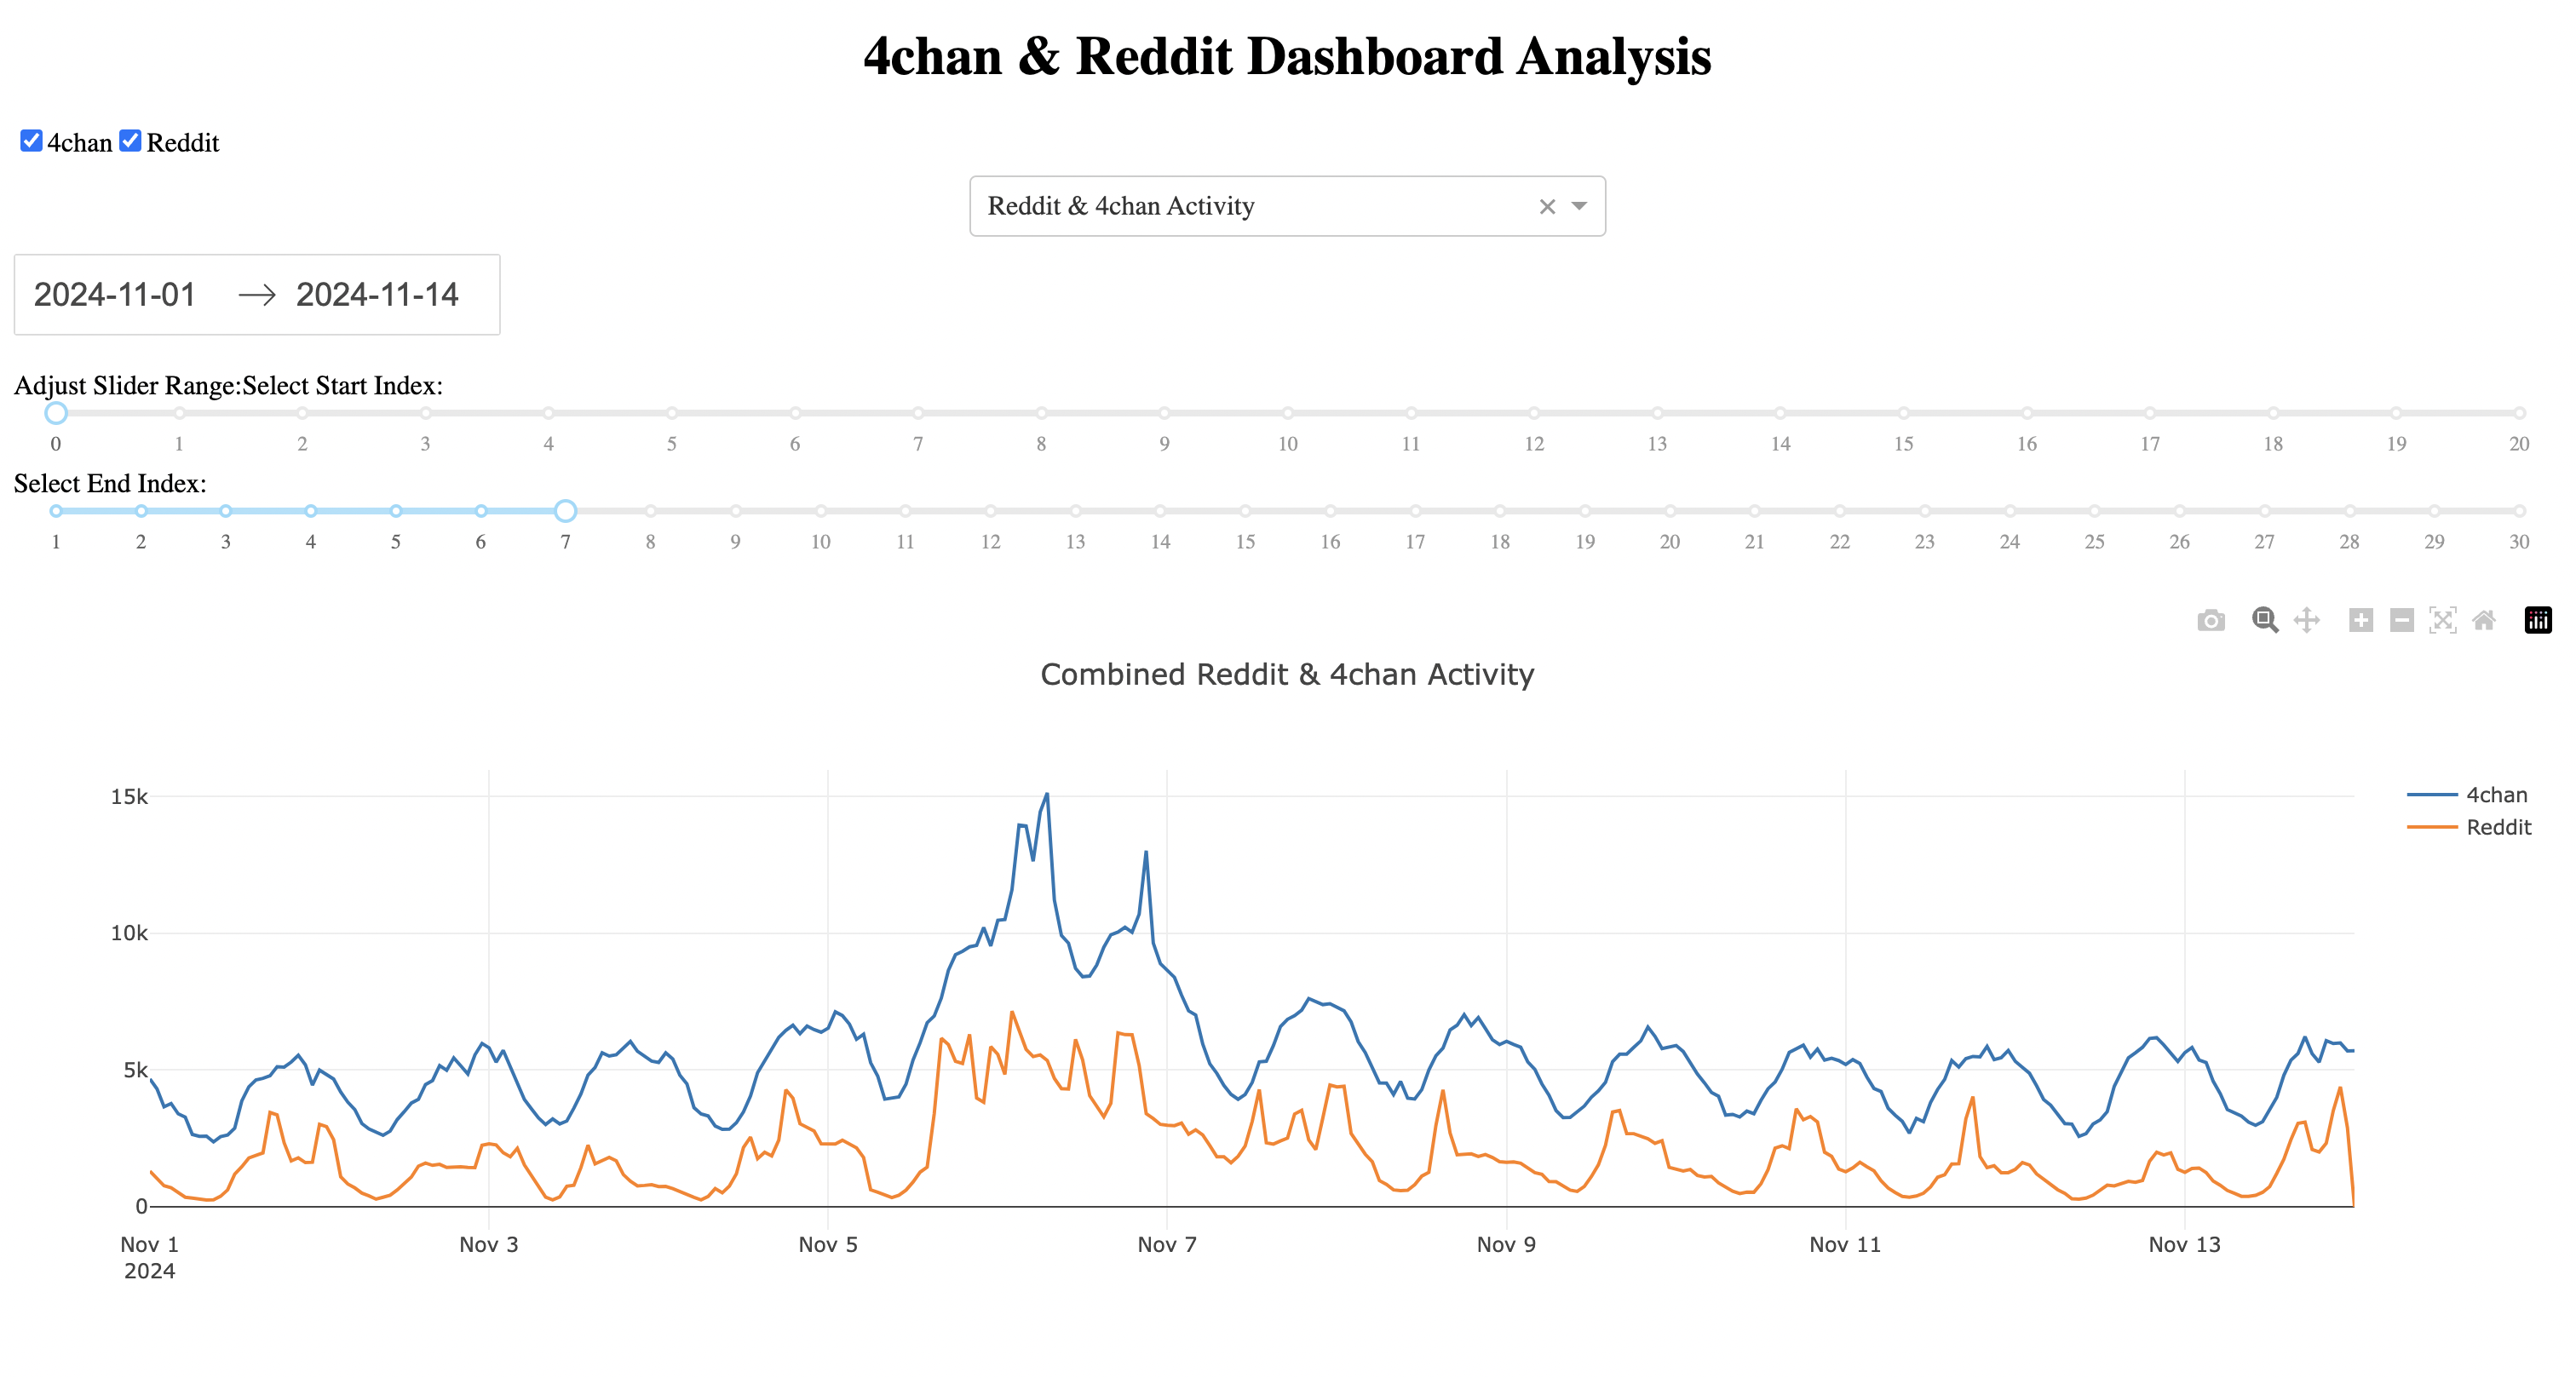
\includegraphics[width=\linewidth]{image.png}
    \caption{Sentimental analysis}
    \label{fig:toxicity_distribution}
\end{figure}
The analysis tracks sentiment trends over time on reddit platform, focusing on four distinct emotional categories: angry, happy, hope, and sad, excluding neutral comments. The data shows the number of comments associated with each sentiment on specific dates in November 2024. From the graph, it's evident that hope and angry sentiments have similar and the highest number of comments throughout the period, with noticeable spikes occurring between November 5th and 7th, 2024. Following these, happy comments show a moderate increase, while sad comments consistently remain at a lower level, with only minor fluctuations.The spikes between November 5th and 7th suggest significant events or occurrences that triggered strong emotional responses, particularly from those expressing hope and anger. This provides valuable insights into the emotional engagement and reactions of the audience during this specific time frame. The sentiment analysis uses keyword-based categorization to classify comments, and the line graph effectively visualizes how each sentiment varied over time. This trend analysis helps understand emotional dynamics in response to events, providing useful data for assessing public mood or engagement.


\begin{figure}[h]
    \includegraphics[width=\linewidth]{download (2) 2.png}
    \caption{Number of comments per hour on Reddit}
    \label{fig:daily_submissions}
\end{figure}
This graph represents the number of comments per hour from November 1 to November 14, 2024, and provides insights into temporal activity patterns. Here's the analysis:

Key Observations:

Major Spike on November 6:

A significant surge in comments is observed on November 6, with the number exceeding 14,000 comments per hour at its peak. This aligns with a major political or social event that drove intense user engagement.
Periodic Cycles:

There is a noticeable periodic pattern, likely reflecting daily activity cycles. Peaks generally occur during specific times of the day, probably corresponding to high-activity hours, while troughs align with periods of lower user activity (e.g., late night).


Activity Before and After November 6:

Before the November 6 peak, the comment activity is relatively stable with smaller fluctuations.
Following the spike, the activity decreases but continues to display the periodic daily pattern.


Sustained Decline Post-Peak:

After November 6, while the hourly comment count gradually decreases, the cyclical nature remains consistent.



\begin{figure}[h]
    \includegraphics[width=\linewidth]{download (3).png}
    \caption{Sentiment analysis excluding neutral on 4Chan}
    \label{fig:hourly_comments}
    
\end{figure}
The analysis tracks sentiment trends over time on 4chan platform, focusing on four distinct emotional categories: angry, happy, hope, and sad, excluding neutral comments. The data shows the number of comments associated with each sentiment on specific dates in November 2024. From the graph, it's evident that hope and angry sentiments have similar and the highest number of comments throughout the period, with noticeable spikes occurring between November 5th and 7th, 2024. Following these, happy comments show a moderate increase, while sad comments consistently remain at a lower level, with only minor fluctuations.The spikes between November 5th and 7th suggest significant events or occurrences that triggered strong emotional responses, particularly from those expressing hope and anger. This provides valuable insights into the emotional engagement and reactions of the audience during this specific time frame. The sentiment analysis uses keyword-based categorization to classify comments, and the line graph effectively visualizes how each sentiment varied over time. This trend analysis helps understand emotional dynamics in response to events, providing useful data for assessing public mood or engagement.


\begin{figure}[h]
    \includegraphics[width=\linewidth]{download (4).png}
    \caption{Election Narratives from comments}
    \label{fig:toxicity_distribution}
\end{figure}
The bar graph represents the frequency of election-related narratives found in comments, with each bar corresponding to a specific narrative. The "red wave" narrative, associated with keywords like "Republican wave," "GOP wave," and "Trump," is the most prominent, as evidenced by the significantly taller red bar. This suggests that discussions around the Republican Party's success or rise in the election were far more prevalent than those around other narratives, indicating a stronger focus on Republican-related topics in the analyzed comments. In contrast, the "blue wave" narrative, linked to keywords such as "Democratic wave," "Dems wave," and "Harris," is represented by a much shorter blue bar, showing that there was comparatively less discussion about the Democratic Party's success in the election. Furthermore, the "split government" narrative, depicted by the green bar, is nearly negligible, highlighting that the concept of a divided government or political gridlock was scarcely mentioned. This analysis suggests a clear emphasis on Republican-related election narratives, with minimal attention given to Democratic or bipartisan issues.



\begin{figure}[h]
    \includegraphics[width=\linewidth]{image (3).png}
    \caption{4Chan vs Reddit DB comparison}
    \label{fig:hourly_comments}
\end{figure}
The graph shows that 4chan’s post count is consistently double that of Reddit from November 1 to November 14, 2024. This could be attributed to 4chan's anonymous, unmoderated environment, which tends to foster higher engagement, especially on politically charged topics. Users on 4chan may feel less restricted, leading to more frequent posts compared to Reddit, where moderation and community guidelines might limit certain types of discussions.

This trend suggests that 4chan's user base is more actively engaged in political discourse during this period, likely due to the 2024 U.S. elections. The higher post volume on 4chan might also indicate a more intense or immediate reaction to current events, while Reddit's more diverse range of discussions could explain its lower post count.


\begin{figure}[h]
    \includegraphics[width=\linewidth]{newplot (2).png}
    \caption{World Map from data}
    \label{fig:daily_submissions}
\end{figure}
The analysis visualizes the top 15 countries with the most comments, excluding the United States, using a choropleth map. The countries are color-coded based on the number of comments, with the highest values represented in blue, the lowest in deep brown, and mid-range values in white. Canada has the highest comment count, followed by other countries in the dataset. The map offers a geographical view of where the most comments are coming from, highlighting regions with significant engagement. The color scale effectively differentiates countries with varying comment counts, with the darkest shades representing countries with fewer comments and the brightest shades indicating higher comment activity. This analysis provides insights into global comment trends, emphasizing international participation and engagement beyond the United States.


\begin{figure}[h]
    \includegraphics[width=\linewidth]{image (1).png}
    \caption{Cumulative Distribution Function (CDF) of comment lengths}
    \label{fig:hourly_comments}
\end{figure}
    The figure depicts the Cumulative Distribution Function (CDF) of comment lengths within the range of 0 to 1000 characters. The x-axis represents the length of the comments, while the y-axis shows the cumulative probability, indicating the fraction of comments that are less than or equal to a given length.

From the CDF curve, we can observe the following:

- Early steep rise: There is a rapid increase in the cumulative probability as the comment length grows from 0 to around 200 characters. This suggests that the majority of the comments are relatively short, with a significant portion of the data being concentrated in the lower end of the length spectrum.
  
- Slower increase after 200 characters: The curve begins to flatten after reaching around 200 characters, indicating that longer comments (those closer to 1000 characters) are less common, and the growth rate of comment length slows down as the distribution progresses.

- Asymptote near 1: The curve approaches 1, which signifies that almost all comments fall within the 0 to 1000 character range, with a very small number of exceptions.

Overall, this distribution suggests that most comments are relatively brief, and only a small proportion of comments extend beyond the 200-character mark, providing insights into the general behavior of the comment lengths within this dataset. This information can help in understanding the level of detail in user responses, indicating that the audience tends to provide shorter comments on average.



\begin{figure}[h]
    \includegraphics[width=\linewidth]{image (2).png}
    \caption{daily count of submissions in a political subreddit (r/politics)}
    \label{fig:daily_submissions}
    \end{figure}
    This graph shows the daily count of submissions in a political subreddit (r/politics) from November 1 to November 14, 2024. Here’s the analysis:

Significant Peak on November 6:

The graph exhibits a sharp spike on November 6, with submissions exceeding 120,000. This suggests a major political event, likely driving intense activity and engagement on this date.
Trend Before and After the Peak:

Submissions were relatively stable from November 1 to November 3, hovering around 40,000 daily.
A gradual increase begins on November 4 and peaks on November 6.
After November 6, there is a steep decline in activity, with submissions progressively decreasing each day.
Smaller Spike Around November 13:

A minor rebound in activity is seen around November 13, possibly due to a related or secondary political event.
Overall Decrease Post-Peak:

After the major spike, the overall trend indicates a decline in engagement as the event's impact likely waned.




\begin{figure}[h]
    \includegraphics[width=\linewidth]{1-graph_visualiser-1733275463228.png}
    \caption{Time series trend of "post count" over the first two weeks of November 2024}
    \label{fig:toxicity_distribution}
    \end{figure}
    The graph below illustrates a time series trend of "post count" over the first two weeks of November 2024. 
    
    Here is an analysis of the pattern observed: 
    
    Cyclic Pattern: The graph exhibits a clear periodicity, with peaks and troughs occurring regularly over the time range. This suggests a repeating daily or weekly cycle in the data. Peak Activity: The highest point occurs around November 6, indicating a surge in post count at that time. This could signify a significant event or trend that caused increased activity. Low Activity: Troughs are consistently observed after each peak, with the post count falling sharply to its lowest levels, likely during off-peak hours. General Trend: Beyond the cyclic nature, the overall trend appears relatively stable, oscillating around a similar range with no evident increasing or decreasing pattern over the time period.



\begin{figure}[h]
    \includegraphics[width=\linewidth]{toxicity.png}
    \caption{Toxicity of countries against count}
    \label{fig:hourly_comments}
    \end{figure}
    The graph shows the number of posts with the "flag" score from 4chan and Reddit over time. When you look at the graph, you'll notice that the U.S. (United States) has the highest number of flagged posts compared to other countries. This suggests that, during the observed period, users from the U.S. were the most active in posting flagged content on these platforms. This could reflect higher engagement or a stronger reaction to political discussions or events, especially considering the context of the 2024 U.S. elections. The data highlights the prominence of U.S. users in the political discourse on these platforms.


\begin{table}
    \centering
    \begin{tabular}{ccc}
       Dataset & Entries Count & Board&\\
       Reddit  & 2249215 & politics&\\
       4Chan  & 3126247 & pol &\\
    \end{tabular}
    \caption{Dataset Details}
    \label{tab:my_label}
\end{table}
Above table represents our dataset sizes and the board which we utilized for data collections.


\subsection{Research Questions}
\begin{enumerate}
     \item How do temporal patterns in social media activity correlate with engagement metrics like comments?
    \item How do shifts in sentiment metrics—such as happy, sad, angry, and hopeful correlate with key events and discussions in U.S. politics ?
    \item How do the tones and volumes of discussions differ between mentions of different political candidates or parties?
\end{enumerate}




\subsection{Limitations}

This section discusses some key limitations encountered in the project:

\begin{itemize}

    \item \textbf{Server Reboot and Downtime:} Due to server reboot and authentication issues, we experienced data loss as the Postgres and Faktory servers were stopped, and even the Docker containers were exited. This caused interruptions in the data processing pipeline and loss of intermediate results.

    \item \textbf{Incomplete Data Coverage:} The datasets may not fully represent all relevant user activities or toxic behavior patterns, as the data is limited to specific subreddits (\texttt{r/politics}) and boards (\texttt{/pol/}) over a short time frame. Important platforms or communities outside the scope of these datasets might provide different insights.
    
    \item \textbf{Potential Bias in Sampling:} The data collection process may introduce sampling bias due to filters or parameters used (e.g., focusing only on specific time windows or content types).

    \item \textbf{Bias in Toxicity Scoring Models:} The ModerateHatespeech API might reflect cultural, linguistic, or contextual biases, leading to inaccuracies in toxicity measurements for certain groups or content types. Toxicity scoring and analysis involve ethical considerations, as incorrectly labeling content or users might lead to stigmatization or misrepresentation.
    
    \item \textbf{Overgeneralization of Results:} Insights derived from this project might not generalize to other social media platforms or communities, as user behavior and moderation policies differ widely across platforms.

    \item \textbf{Limited Computational Resources:} Large datasets and real-time scoring might be computationally intensive, leading to delays or scalability challenges when expanding the scope.
    
    \item \textbf{Data Storage and Loss:} Redundancy was implemented, but issues with storage capacity or processing errors might have caused partial data loss.

    
\end{itemize}


\subsection{Future Work}
To enhance usability and accessibility, we plan to develop a web-based interactive dashboard. This tool will allow users to query the data and visualize results from the analyses conducted in this project. The dashboard will enable intuitive exploration and comparison of datasets. It also involves deeper exploration of research questions and integration of additional datasets.



\section{Conclusion}
This project demonstrates the integration of real-time toxicity scoring into a social media data pipeline and highlights insights into activity and toxicity trends. The results lay the groundwork for answering research questions in the next phase of the project.

\subsection{Problems faced}
As VM went down multiple times our hate speech api scores were not enough to reach a satisfactory conclusions.

\section{References}
\begin{enumerate}
    \item ModerateHatespeech API Documentation. \url{https://moderatehatespeech.com}.
    \item ACM Proceedings Template. \url{https://www.acm.org/publications/proceedings-template}.
    \item 
    \url{https://brightspace.binghamton.edu/d2l/le/content/360366/viewContent/1227658/View}
    \item 
    \url{https://brightspace.binghamton.edu/d2l/le/content/360366/viewContent/1227668/View}
    \item
    \url{https://brightspace.binghamton.edu/d2l/le/content/360366/viewContent/1227669/View}
\end{enumerate}



\end{document}